\clearpage{}
\section{Source language and constraint slurping}
\label{Inference:Language}

This section presents the formal description of our desugared source language and discusses how to generate type constraints. The typing rules given in this chapter serve as inspiration when generating constraints, but correctness for our overall system relies on the proof of soundness for the core language given in the appendix.

Any errors in constraint generation or type inference will be detected when checking the program once it has been translated to core. We believe this is a fair approach, because new type systems are usually presented for a cut down, desugared language anyway. We view the core type system as the ``real'' type system for Disciple, with the system presented in this chapter being part of the compiler implementation. 


\bigskip
\bigskip
% -- Declarations
\subsubsection{Declarations}
\vspace{-1ex}
\begin{tabbing}
MM 	\= MM \= MMMMMMMMMMMMMMMMMMMM \= MMMMMMM \kill
$\ipgm$	\>   $\to$	\> $\ov{\idecl}; \ t$						\> (program)		\\[1ex]
$\idecl$ 
	\>   $\to$ 	\> $\kdata \ T :: \% \to \ov{\kappa} \to * \ \kwhere \ \ov{K : \varphi}$ 
			\> (data type declaration)
\end{tabbing}

Programs consist of a list of declarations followed by a term to be evaluated. Data type declarations introduce a new type constructor $T$, and give its kind. All type constructors $T$, and data constructors $K$ defined in a program must be distinct. We define the meta-function ctorTypes($T$) to get the list of data constructors $\ov{K : \varphi}$ corresponding to a particular type constructor $T$.

The set of allowable types for data constructors is more restrictive than indicated here. These restrictions are introduced by the typing rules presented in \S\ref{inference:language:declarations}.



\bigskip
\bigskip
% -- Kinds ----------------------
\subsubsection{Kinds}
\vspace{-2ex}
\begin{tabbing}
MM 	\= MM \= MMMMMMMMMMMMMMMMMMMM \= MMMMMMM \kill
$\kappa$ 
	\>   $\to$ 	\> $(\kappa_1 \to \kappa_2)$ 	  				\> (kind function)	\\
 	\> \ $\mid$	\> $* \ \mid \ \% \ \mid \ ! \ \mid \ \$$ 			\> (atomic kind constructors)
\end{tabbing}

Kinds consist of kind functions and the atomic kinds $*$, $\%$, $!$ and $\$$ which are the kinds of value types, regions, effects and closures respectively. 




\clearpage{}
% -- Types ---------------------
\vspace{-2em}
\subsubsection{Types}
\vspace{-1ex}
\begin{tabbing}
MM 	\= MM \= MMMMMMMMMMMMMMMMMM \= MMMMMMM \kill
$\varphi$, $\tau$, $\sigma$, $\varsigma$	\\
	\> $\to$	\> $a_\kappa$					\> (type variables) \\
	\> \ $\mid$	\> $\varphi \ \rhd \ \Omega$			\> (constrained type) \\
	\> \ $\mid$	\> $\forall (a : \kappa). \ \varphi$		\> (unbounded quantification) \\
	\> \ $\mid$	\> $\varphi_1 \lor \varphi_2$			\> (least upper bound) \\
	\> \ $\mid$	\> $\top_\kappa \ \ \mid  \ \ \bot_\kappa$	\> (top and bottom) \\
	\> \ $\mid$	\> $\tau_1 \lfuna{\sigma \ \varsigma} \tau_2$	\> (function type constructor) \\
	\> \ $\mid$	\> $T_{\kappa} \ r \ \ov{\varphi}$		\> (data type constructor) \\
	\> \ $\mid$	\> $\iRead \ r \ 
				\ \mid \ \iReadH \ \tau \ 
				\ \mid \ \iWrite \ r$ 		\> (effect type constructors) \\
	\> \ $\mid$	\> $x : \varphi$				\> (closure constructor)
\end{tabbing}

We do not make a rigid syntactic distinction between polytypes and monotypes, or constrained and unconstrained types. For this we are inspired by the pure type system approach of the lambda cube and the Henk intermediate language \cite{peyton-jones:henk}. We also do not make a syntactic distinction between value types, regions, closures and effects. We have found maintaining these distinctions to be cumbersome in both the presentation and implementation. However, we will hint at the intended kind of a particular type by using the variables $\varphi$, $\tau$, $\sigma$ and $\varsigma$. We intend $\tau$ to be an unquantified value type, $\sigma$ and $\varsigma$ to be unquantified effect and closure types respectively, and allow $\varphi$ to be any type. $a_k$ are type variables tagged with their kind, though we tend to elide their kinds in this presentation. As type variables contain their kinds, we can determine the kind of an arbitrary type expression without needing an auxiliary environment. When a specific kind is intended we use $s$, $r$, $e$ and $c$ as value type, region, effect and closure variables respectively.

$\Omega$ is a set of constraints. The term $\varphi \rhd \Omega$ is a constrained type whose general meaning is similar to $\Omega \Rightarrow \varphi$ in Haskell style systems deriving from type classes \cite{wadler:less-ad-hoc} and Jones's work on general qualified types \cite{jones:qualified-types}. The expression $\varphi \rhd \Omega$ is pronounced ``$\varphi$ with $\Omega$''. We use the $\varphi \rhd \Omega$ form because we find it easier to read when there are a large number of constraints, and the order of constraints in the source language is irrelevant. Although $\Omega$ is a set, we usually write $\varphi \rhd \chi_1, \chi_2$ instead of $\varphi \rhd  \{ \chi_1, \chi_2 \}$. We take $\varphi \rhd \emptyset$ as being equivalent to $\varphi$. 

We use only unbounded quantification in the source language. In the type $\forall (a : \kappa). \varphi$ we usually elide the kind term when it is obvious from the name of the variable. For example, $\forall r_1. \varphi$ quantifies a region variable and $\forall e_1. \varphi$ quantifies an effect variable. We treat $\forall \ov{a : \kappa}. \ \varphi$ as short for $\ov{\forall a : \kappa}. \ \varphi$. We also treat expressions like $\forall r_{1..3}. \ \varphi$ as short for $\forall r_1 \ r_2 \ r_3. \ \varphi$. The operator $\rhd$ binds more tightly than $\forall$, so the type $\forall (a : \kappa). \ \varphi \rhd \Omega$ should be read as $\forall (a : \kappa). \ (\varphi \rhd \Omega)$. We do not consider higher ranked types, and assume that all quantified types are in prenex form.

The least upper bound $\varphi_1 \lor \varphi_2$ is defined on effect and closure types only. $\top_\kappa$ and $\bot_\kappa$ include their kinds and $\top$ may only be an effect. In the types presented to the user, $\bot_\kappa$ may be an effect or closure only, but during type inference we abuse the notation and use it as a value type and region type as well. The function type $\tau_1 \lfuna{\sigma \ \varsigma} \tau_1$ contains effect and closure annotations, but if these are not present we will assume they are $\bot$. Due to the form of the data type definitions, data type constructors $T_{\kappa} \ r \ \ov{\varphi}$ always have their primary region variable as as their first parameter. The $\kappa$ in the subscript is the constructor's kind. 

$\iRead r$, $\iReadH \tau$ and $\iWrite r$ are our initial effect types, though we will add more later. $\iReadH \tau$ expresses a read on a data constructor's primary region, and we use it when generating type constraints for case expressions. $x : \varphi$  is a closure term tagged with a usefully named value variable. See \S\ref{System:Closure} for a discussion of this.



\bigskip
\bigskip
% -- Constraints
\vspace{-2em}
\subsubsection{Constraints}
\vspace{-1ex}
\begin{tabbing}
MM 	\= MM \= MMMMMMMMMMMMMMMMMMM \= MMMMMMM \kill
$\chi$ 	\> $\to$	\> $\tau_1 = \tau_2$				\> (type equality) \\
	\> \ $\mid$	\> $\varphi_1 \tme \varphi_2$				\> (effect or closure constraint)
\end{tabbing}

Our initial type constraints are $\tau_1 = \tau_2$ and $\varphi_1 \tme \varphi_2$, though we will add type class constraints later. Equality constraints like $\tau_1 = \tau_2$ are used to constrain value types and type variables of all kinds. Inequality constraints like $\varphi_1 \tme \varphi_2$ are used to constrain effects and closures. When performing type checking we must allow the left of these constraints to be a full type, though in annotations and type schemes it is always a variable. When performing type inference and checking, all effect and closure constraints must be in the weak form discussed in \S\ref{System:Effects:constraint-strengthening}. Types are strengthened only when presenting them to the user or converting them to the core language.



\bigskip
\bigskip
% -- Terms
\vspace{-2em}
\subsubsection{Terms}
\vspace{-1ex}
\begin{tabbing}
MM 	\= MM \= MMMMMMMMMMMMMMMMMMMM \= MMMMMMM \kill
$t$ 	\> $\to$ 	\> \ $x$						\> (term variable) 	\\
	\> \ $\mid$	\> \ $K$						\> (data constructor)	\\
	\> \ $\mid$	\> \ $\lambda x. \ t$					\> (term abstraction) 	\\
	\> \ $\mid$	\> \ $t_1 \ t_2$					\> (term application) 	\\
	\> \ $\mid$	\> \ $\rblet \ \ov{x = t} \ \rbin \ t'$		\> (let bindings) 	\\
	\> \ $\mid$	\> \ $\kcase \ t \ \kof \ \ov{p \to t'}$		\> (case expression) 
\end{tabbing}

% -- Patterns
\vspace{-2em}
\subsubsection{Patterns}
\vspace{-1ex}
\begin{tabbing}
MM 	\= MM \= MMMMMMMMMMMMMMMMMMMM \= MMMMMMM \kill
$p$ 	\> $\to$ 	\> \ $\_$						\> (wild card) \\
	\> \ $\mid$	\> \ $K \ \ov{x}$					\> (constructor pattern) 
\end{tabbing}

% -- Derived Forms
\vspace{-2em}
\subsubsection{Derived Forms}
\vspace{-1ex}
\begin{tabbing}
MM	\= MMMMMMMMMMMMM \= MMMMMM \kill	
	\> $\kif \ t_1 \ \kthen \ t_2 \ \kelse \ t_3$
		\> $\equalsdef \ \kcase \ t_1 \ \kof \ \{ \iTrue \to t_2; \ \iFalse \to t_3 \}$ 
	\\[2ex]

	\> $\kdo \ \ov{\ibindstmt} \ ; \ t$
		\> $\equalsdef \ \klet \ \ov{\trm{mkBind}(\ibindstmt)} \ \kin \ t$
	\\[1ex]
	\> \trm{where} $\ibindstmt$		\> $\to \ x = t \ \mid \ t$ 
	\\
	\> \hspace{2.6em} $\trm{mkBind}(x = t)$	\> $\equalsdef \ x = t$ \\
	\> \hspace{2.6em} $\trm{mkBind}(t)$ 	\> $\equalsdef \ x = t, \ \ x \ \trm{fresh}$ 
\end{tabbing}

Our term language is standard, with let bindings being mutually recursive. This is only a simple desugared language. Full Disciple is sweeter and includes pattern guards, kind inference, monadic do notation, and other features --- but we do not discuss them here.


\clearpage{}
% -------------------------------------------------------------------------
\subsection{Normal types}
\label{inference:language:normal-types}

Although the language definition provides a high degree of freedom when writing type expressions, the types presented to the programmer are all \emph{normal}.


Consider the following type:

\code{
	$succ$ 	& \mc{2}{$:: \forall e_1 \ r_1 \ r_2. \ \iInt \ r_1 \lfuna{e_1} \iInt \ r_2$} \\
		& $\rhd$	& $e_1 \tme \iRead \ r_1$
}

We could also write this as:

\code{
	$succ$ 	& \mc{2}{$:: \forall e_1 \ r_1 \ r_2. \ s_1 \lfuna{e_1} s_2$} \\
		& $\rhd$ 	& $s_1 = \iInt \ r_1$ \\
		& \ $,$		& $s_2 = \iInt \ r_2$ \\
		& \ $,$		& $e_1 \tme \iRead \ r_1$
}

\quad or:

\code{
	$succ$ 	& \mc{2}{$:: \forall e_1 \ r_1 \ r_2.\ (s_1 \rhd s_1 = \iInt \ r_1) \lfuna{e_1} s_2$} \\
		& \ $\rhd$		& $s_2 = \iInt \ r_2$ \\
		& \ $,$		& $e_1 \tme \iRead \ r_1$
}

All three of these types are equivalent, and perfectly valid in our system, though only the first is normal. The last two can appear as intermediate forms during type inference. Normal types obey the following rules:
\begin{enumerate}
\item	Normal types are of the form $\forall \ov{a : \kappa}. \ \varphi \rhd \Omega$ where $\varphi$ 
	is not another constrained type like $\varphi_1 \rhd \Omega$. When this restriction is in place
	we refer to $\varphi$ as the \emph{body} of the type.

\item	There are no $\tau_1 = \tau_2$ constraints, and the left positions of all $\varphi_1 \tme \varphi_2$
	constraints are variables.

\item	For every constraint set $\Omega$ in the type, there is only one constraint per variable.
	For example, we write $\varphi \rhd e \tme \sigma_1 \lor \sigma_2$ instead
	of $\varphi \rhd e \tme \sigma_1, \  e \tme \sigma_2$.


\item	Normal types do not contain nested closure terms of the form $x_1 : x_2 : \varphi$. The value variables
	are used for documentation only, so we keep just the first one and write $x_1 : \varphi$ instead.
\end{enumerate}


\clearpage{}
% -----------------------------------------------------------------------------
\subsection{Free variables of types}
\label{Inference:Language:free-variables}
The function for computing the free variables of a type is unsurprising:

\bigskip
\code{
	$\ifv(a)$	
		& $= \{ a \}$ 
	\\[1ex]
	$\ifv(\varphi \rhd \Omega)$
		& $= \ifv(\varphi) \setminus \{ a \ | \ (a = \varphi') \in \Omega \}$
	\\[1ex]
	$\ifv(\forall(a : \kappa). \ \varphi)$
		& $= \ifv(\varphi) \setminus \{ a \}$
	\\[1ex]
	$\ifv(\varphi \lor \varphi')$
		& $= \ifv(\varphi) \cup \ifv(\varphi')$
	\\[1ex]
	$\ifv(\bot)$
		& $= \emptyset$
	\\[1ex]
	$\ifv(\top)$
		& $= \emptyset$
	\\[1ex]
	$\ifv(\tau \lfuna{\sigma \ \varsigma} \tau')$
		& $= \ifv(\tau) \cup \ifv(\tau') \cup \ifv(\sigma) \cup \ifv(\varsigma)$
	\\[1ex]
	$\ifv(T_\kappa \ r \ \ov{\varphi})$
		& $= \{ r \} \cup \ov{\ifv(\varphi)}$
	\\[1ex]
	$\ifv(\iRead \ r)$
		& $= \{ r \}$
	\\[1ex]
	$\ifv(\iReadH \ \tau)$
		& $= \ifv(\tau)$
	\\[1ex]
	$\ifv(\iWrite \ r)$
		& $= \{ r \}$
	\\[1ex]
	$\ifv(x : \varphi)$
		& $= \ifv(\varphi)$
}

\bigskip
\bigskip
\bigskip
\bigskip
% -----------------------------------------------------------------------------
\subsection{Dangerous variables}
\label{Inference:Language:dangerous-variables}
Dangerous variables were discussed in \S\ref{System:Closure:dangerous}. To compute the dangerous variables of a type we use a domain $D$, where a member of this domain can be either a pair consisting of a set of constraints and a type expression $\apair{\{\chi\}, \varphi}$, or a dotted type variable $a^\bullet$.

\code{
	$D = \{ \text{Constraint} \} \times \text{Type} \ + \ \text{DotVar}$
}

To compute the dangerous variables in a particular type $\varphi$, we start with the set $\{ \apair{\emptyset, \varphi} \}$ then iteratively apply the relation $dv : \{ D \} \to \{ D \}$ until we reach a fixpoint. In the resulting set, the dotted variables are the ones that are dangerous in the initial type.

\clearpage{}
The relation $\idv$ is as follows:

\code{
	$\idv : \{ D \} \to \{D\}$ 
	\\[1ex]
	$\idv(\mu) = \mu \ \cup \ \bigcup\{ \idv'(x) \ | \ x \in \mu \}$ \\
}

where

\code{
	$\idv' : D \to \{D\}$
	\\[1ex]
	$\idv' ( a^\bullet )$
		& $= \{ a^\bullet \}$
	\\[1ex]
	$\idv' ( \apair{\Omega, \ a} )$
		& $= \emptyset$
	\\[1ex]
	$\idv' ( \apair{\Omega, \ \varphi \rhd \Omega'} )$
		& $= \{ \apair{\Omega \cup \Omega', \ \varphi} \}$
	\\[1ex]
	$\idv' ( \apair{\Omega, \ \varphi \lor \varphi'} )$	
		& $= \{ \apair{\Omega, \ \varphi}, \ \apair{\Omega, \ \varphi'} \}$
	\\[1ex]
	$\idv' ( \apair{\Omega, \ \bot} )$	
		& $= \emptyset$ 
	\\[1ex]
	$\idv' ( \apair{\Omega, \ \top} )$	
		& $= \emptyset$ 
}

\vspace{-1ex}
\code{
	\mc{3}{$\idv' (\apair{\Omega, \ \tau \lfuna{\sigma \ c} \tau'})$} 
		& $= \{\apair{\Omega, \ \varphi}\}$ \\
	\qq $\kwhere$	& $(c \tme \varphi) \in \Omega$
}

\vspace{-1ex}
\code{	
	\mc{4}{$\idv' (\apair{\Omega, \ T_{\kappa} \ r \ \ov{\varphi}})$}  \\
		& $| \ \iMutable \ r \in \Omega$ 
			& $= \{ a^\bullet \ | \ a \in \ifv(\ov{\varphi}) \} $  \\
		& $| \ \iotherwise$ 
			& $= \{ \apair{\Omega, \tau[r \ \ov{\varphi} / \ov{a}]} \ 
					| \ \forall \ov{a}. \ \tau \in \iargs(\ictorTypes(T)) \}$
}

\vspace{-1ex}
\code{
	$\idv' (\apair{\Omega, \ \iRead \ r})$
		& \quad $= \emptyset$
	\\[1ex]
	$\idv' (\apair{\Omega, \ \iReadH \ \tau})$
		& \quad $= \emptyset$
	\\[1ex]
	$\idv' (\apair{\Omega, \ \iWrite \ r})$
		& \quad $= \emptyset$
	\\[1ex]
	$\idv' (\apair{\Omega, \ x : \varphi})$	
		& \quad $= \{\apair{\Omega, \ \varphi}\}$ 
}

The $\ictorTypes$ function returns the types of the constructors associated with a particular data type constructor $T$. The $\iargs$ function returns the arguments of these constructors, retaining the outer quantifiers. As we only compute the dangerous variables of a type \emph{before} generalising it, there is no need to match on the $\forall (a : \kappa). \varphi$ form. If we take the sets $\{ D \}$ to be ordered by set inclusion, the function $\idv$ is monotonic by construction, as it always returns its argument as part of the result.

For example, suppose the type $\iTwoThings$ is defined as:

\code{
	\mc{3}{$\kdata \ \iTwoThings \ r_{1..3} \ a \ b$} \\
	& =	& $T1 \ (\iMaybe \ r_2 \ a)$ \\
	& \ $|$	& $T2 \ (\iMaybe \ r_3 \ b)$ \\
}

In the desugared language this becomes:

\code{
	\mc{3}{$\kdata \ \iTwoThings \ r_{1..3} \ a \ b \ \kwhere$} \\
	& $\iTOne :: \forall r_{1..3} \ a \ b. \ \iMaybe \ r_2 \ a \to \iTwoThings \ r_{1..3} \ a \ b$ \\
	& $\iTTwo :: \forall r_{1..3} \ a \ b. \ \iMaybe \ r_3 \ b \to \iTwoThings \ r_{1..3} \ a \ b$ 
}

Now, if $r_1$ was mutable, then we could update both alternatives, so both $a$ and $b$ would be dangerous. However, if $r_2$ was mutable then $a$ would be dangerous (but not necessarily $b$), and if $r_3$ was mutable then $b$ would be dangerous (but not necessarily $a$). 

With this definition, the value of $\iargs(\ictorTypes(\iTwoThings))$ is:

\code{
	$\{ \forall r_{1..3} \ a \ b. \iMaybe \ r_2 \ a, \ \forall r_{1..3} \ a \ b. \iMaybe \ r_3 \ b \ \}$
}

Suppose we wish to determine the dangerous variables in the type:

\code{
	$\iTwoThings \ r_4 \ r_5 \ r_6 \ (\iInt \ r_7) \ (c \to d) \rhd \iMutable \ r_5$
}

The following is the sequence of states we get when computing the fixpoint. We save space by writing $...$ in place of the elements of the previous state.

\code{
		  & $\{ \apair{\emptyset, \iTwoThings \ r_4 \ r_5 \ r_6 \ (\iInt \ r_7) \ (c \to d) \rhd \iMutable \ r_5} \}$
\\[2ex]
	$\vdash$  & $\{ ..., \ \apair{ \{\iMutable \ r_5 \}, \ \iTwoThings \ r_4 \ r_5 \ r_6 \ (\iInt \ r_7) \ (c \to d)} \}$
\\[2ex]
	$\vdash$  & $\{ ..., \ \apair{ \{\iMutable \ r_5 \}, \ \iMaybe \ r_5 \ (\iInt \ r_7) }$ \\
		  & \quad \  $, \ \apair{ \{ \iMutable \ r_5 \} , \ \iMaybe \ r_6 \ (c \to d)} \ \}$
\\[2ex]
	$\vdash$  & $\{ ..., \ r_7^{\ \bullet}, \ c \to d \}$
}

Hence, only $r_7$ is dangerous. The variables $c$ and $d$ would only be dangerous if $r_6$ or $r_4$ were mutable.

Computing the dangerous variables of a type using a fixpoint allows us to deal with recursive types. For example, the list type has the following desugared definition:

\code{
	\mc{4}{$\kdata \ \iList \ r_1 \ a \ \kwhere$} \\
	& $\iNil$ 	& $::$ 	 & $\forall r_1 \ a. \iList \ r_1 \ a$ 
	\\[1ex]
	& $\iCons$	& $::$ 	 & $\forall r_1 \ a \ c_1. \ a \to \iList \ r_1 \ a \lfuna{c_1} \iList \ r_1 \ a$ \\
	&		& $\rhd$ & $c_1 \tme x : a$
}

Here is the sequence of states we get when determining the dangerous variables in the type $\iList \ r_1 \ (\iMaybe \ r_2 \ c) \rhd \iMutable \ r_2$

\medskip
\code{
	 	 & $\{ \apair{\emptyset, \ \iList \ r_1 \ (\iMaybe \ r_2 \ c) \rhd \iMutable \ r_2} \}$
\\[2ex]
	$\vdash$ & $\{ ..., \ \apair{ \{\iMutable \ r_2\}, \ \iList \ r_1 \ (\iMaybe \ r_2 \ c)} \}$
}

Note that when $\idv'$ is applied to the last element in this set, it yields the following pairs:

\code{
	$\{$ 	& $\apair{ \{\iMutable \ r_2\}, \ \iList \ r_1 \ (\iMaybe \ r_2 \ c)}$	\\
	$\ ,$	& $\apair{ \{\iMutable \ r_2\}, \ \iMaybe \ r_2 \ c}$ & $\}$
}

The second element here is new, but the first is was already present in the previous set, and arises due to the recursiveness of the $\iList$ type.

Continuing on with the process, we obtain the following states, with the last one being the fixpoint.

\code{
	$\vdash$ 	& $\{..., \ \apair{\{\iMutable \ r_2\}, \ \iMaybe \ r_2 \ c} \}$
\\[1ex]
	$\vdash$	& $\{..., \ c^\bullet \}$
}

This shows us that the type variable $c$ is dangerous in this type, as expected.


\clearpage{}
% ---------------------------------------------------------
\subsubsection{Problems with nested data types}
Note that a direct implementation of the definition of $\idv$ will diverge when applied to a nested data type \cite{bird:nested-datatypes}.\footnote{Thanks to one of my thesis examiners for pointing this out.} For example, consider the following type:

\code{
	\mc{5}{$\kdata \ \iNest \ r_1 \ a \ \kwhere$} \\
	& $\iMkNest$ & $::$ & $\forall r_1 \ a. \iNest \ r_1 \ (\iList \ r_1 \ a) \to \iNest \ r_1 \ a$
}

This type is considered ``nested'' because the recursive application of $\iNest$ in the first parameter of $\iMkNest$ does not have the same form as that which is being defined, that is, it's not just another $\iNest \ r_1 \ a$. Here is what happens if we try to compute the dangerous variables in the type $\iNest \ r_1 \ a$:

\code{
			& $\{ \apair{\emptyset, \ \iNest \ r_1 \ a} \}$ 
\\[1ex]
	$\vdash$	& $\{..., \apair{\emptyset, \ \iNest \ r_1 \ (\iList \ r_1 \ a}\}$ 
\\[1ex]
	$\vdash$	& $\{..., \apair{\emptyset, \ \iNest \ r_1 \ (\iList \ r_1 \ (\iList \ r_1 \ a))}\}$ 
\\[1ex]
	$\vdash$	& $\{..., \apair{\emptyset, \ \iNest \ r_1 \ (\iList \ r_1 \ (\iList \ r_1 \ (\iList \ r_1 \ a)))}\}$ 
\\[1ex]
	$...$
}

The application of $\idv$ to each successive state yields a larger state, which causes our computation to diverge. However, in the limit, no dotted variables such as $r_1^\bullet$ will be produced, so there are no dangerous variables in the original type. To say this another way: although $\idv$ is sufficient to \emph{define} the set of dangerous variables, it is not sufficient to compute it, if applied in a naive way. 

As mentioned in \cite{bird:nested-datatypes}, the use of nested data types in practice is rare. Also, important generic functions that operate on them (such as $\ifold$) need to be assigned rank-2 types, which we do not support either. We expect that computing the dangerous variables of a nested data type could be done using a reachability analysis instead of direct substitution. However, as checking whether a type is nested or not is straight forward, we have not investigated this further. 


% -----------------------------------------------------------------------------
\subsection{Material and immaterial variables}
\label{inference:material-regions}

The difference between material and immaterial region variables was discussed in \S\ref{System:Closure:shared-regions}. Recall that material region variables correspond to physical objects in the store, whereas immaterial region variables are used to describe the locations of the parameter and return values of functions. In \S\ref{System:Closure:trimming} we discussed how closure terms that do not contain material region variables can be \emph{trimmed} out. In \S\ref{System:Closure:strong-mixed-absent-variables} we defined \emph{strongly material} region variables to be the ones that appear in material positions, but not in immaterial ones. In \S\ref{System:TypeClassing:shape-immaterial} we discussed how the immaterial portions of objects cannot be copied.

The following functions, $\imv$, $\iiv$ are used to compute the material and immaterial variables of a type. The strongly material variables are then obtained by subtracting the second from the first. The type is required to be in normal form, which is described in \S\ref{inference:language:normal-types}. The $\imv$ and $\iiv$ functions are defined similarly to the $\idv$ function from the previous section, and we use the same fixpoint process. Note that we classify isolated value type variables as material because they have the potential to be constrained to a type that contains material region variables, such as $\iInt \ r_1$.


% -- material vars --------------------
\subsubsection{Material Variables}
\code{
	$\imv : \{ D \} \to \{D\}$ 
	\\[1ex]
	$\imv(\mu) = \mu \ \cup \ \bigcup\{ \imv'(x) \ | \ x \in \mu \}$ \\
}

where

\code{
	\mc{2}{$\imv' : D \to \{D\}$}
	\\[1ex]
	\mc{2}{$\imv' ( a_\kappa^\bullet )$} 	
		& $= \{ a_\kappa^\bullet \}$
	\\[1ex]
	\mc{2}{$\imv' ( \apair{\Omega, \ a_\kappa} )$} \\
	& $| \ \kappa \in \{ \%, \ * \}$	& $= \{ a_\kappa^\bullet \}$ \\
	& $| \iotherwise$			& $= \emptyset$
	\\[1ex]
}

\vspace{-1ex}
\code{	
	\mc{4}{$\imv' (\apair{\Omega, \ T_{\kappa} \ r \ \ov{\varphi}})$}  \\
		& $= \{r^\bullet\} \cup \{ \apair{\Omega, \tau[r \ \ov{\varphi} / \ov{a}]} \ 
					| \ \forall \ov{a}. \ \tau \in \iargs(\ictorTypes(T)) \}$ 
	\\[1.5ex]
	\mc{4}{... other cases as per $\idv'$}
}


\bigskip
\bigskip
% -- immaterial vars ------------------
\subsubsection{Immaterial Variables}
\code{
	$\iiv : \{ D \} \to \{D\}$ 
	\\[1ex]
	$\iiv(\mu) = \mu \ \cup \ \bigcup\{ \iiv'(x) \ | \ x \in \mu \}$ \\
}

where

\code{
	\mc{2}{$\iiv' : D \to \{D\}$}
	\\[1ex]
	\mc{2}{$\iiv' ( a_\kappa^\bullet )$} 	
		& $= \{ a_\kappa^\bullet \}$
	\\[1ex]
	\mc{2}{$\iiv' ( \apair{\Omega, \ a_\kappa} )$} \\
	& $| \ \kappa \in \{ \%, \ * \}$	& $= \emptyset$ \\
	& $| \iotherwise$			& $= \{ a_\kappa^\bullet \}$
	\\[1ex]
}

\vspace{-1ex}
\code{
	\mc{4}{$\iiv' (\apair{\Omega, \ \tau \lfuna{e \ c} \tau'})$} \\
		& \mc{3}{$= \{ a^\bullet 
				\ | \ a \in \ifv(\tau) \cup \ifv(\tau') \cup \ifv(\varphi)  \cup \{ e, \ c \} \}
				\ \cup \ \{ \apair{\Omega, \ \varphi'} \}$} \\
	& $\kwhere$	& $(e \tme \varphi) \in \Omega, \ (c \tme \varphi') \in \Omega$
}

\vspace{-1ex}
\code{	
	\mc{4}{$\iiv' (\apair{\Omega, \ T_{\kappa} \ r \ \ov{\varphi}})$}  \\
		& $= \{ \apair{\Omega, \tau[r \ \ov{\varphi} / \ov{a}]} \ 
					| \ \forall \ov{a}. \ \tau \in \iargs(\ictorTypes(T)) \}$
}


\code{
	\mc{2}{$\iiv'(\apair{\Omega, \ \iRead \ r})$}
		& $= \ \{ r^\bullet \}$
	\\[1ex]
	\mc{2}{$\iiv'(\apair{\Omega, \ \iReadH \ \tau})$}
		& $= \ \{ a^\bullet \ | \ a \in \ifv(\tau) \}$ 
	\\[1ex]
	\mc{2}{$\iiv'(\apair{\Omega, \ \iWrite \ r})$}
		& $= \ \{ r^\bullet \}$
	\\[1ex]
	\mc{2}{$\iiv'(\apair{\Omega, \ x : \varphi})$}
		& $= \ \apair{\Omega, \ \varphi}$
	\\[1ex]
	\mc{2}{... other cases as per $\idv'$}
}

\clearpage{}
\subsubsection{Examples:}

\begin{tabbing}
M \= MMMMMMMMMMMMMMMMMMMM \= MMMMM \= MMMMMMM \= MMMMM \kill
	\> $\tau$			
	\> material
	\> immaterial
	\> strongly material
	\\[-1ex]
	\rule{40em}{0.1pt}
	\\
	% -----
	\> $\begin{aligned}
		\iInt \ r_1
	    \end{aligned}$		
	\> $r_1$				
	\> $\emptyset$
	\> $r_1$
	\\[2ex]
	% -----
	\> $\begin{aligned}
		\iList \ r_1 \ a
	    \end{aligned}$
	\> $r_1 \ a$				
	\> $\emptyset$
	\> $r_1 \ a$
	\\[2ex]
	% -----
	\> $\begin{aligned}
		a \to \iInt \ r_1
	    \end{aligned}$
	\> $\emptyset$
	\> $a \ r_1$
	\> $\emptyset$
	\\[2ex]
	% -----
	\> $\begin{aligned}
	 & () \lfuna{e_1 \ c_1} () \\
	 & \quad \rhd	  e_1 \tme \iWrite \ r_3 \\
	 & \quad \ , \ \: c_1 \tme x_1 : \iInt \ r_3 \ \lor \ x_2 : \iInt \ r_4 \\
	 \end{aligned}$\quad\quad
	\> \rule{0ex}{6ex}
	  $r_3 \ r_4$
	\> $e_1 \ c_1 \ r_3$
	\> $r_4$
	\\[4ex]
	% -----
	\> $\begin{aligned}
	 & \iInt \ r_1 \lfuna{e_1 \ c_1} \iInt \ r_2 \\
	 & \quad \rhd e_1 \tme \iRead \ r_1 \\
	 & \quad \ , \ \:  c_1 \tme x : \iInt \ r_2
	 \end{aligned}$ \quad \quad
	\> \rule{0ex}{6ex}
          $r_2$
	\> $r_1 \ r_2 \ e_1 \ c_1$
	\> $\emptyset$ 
	\\
	% -----
	\> $\begin{aligned}
	 & \iMaybe \ r_1 \ (a \lfuna{\bot \ c_1} \iInt \ r_3) \\
	 & \quad \rhd c_1 \tme x : \iInt \ r_3
	 \end{aligned}$ 
	\> \rule{0ex}{6ex}
    	  $r_1 \ r_3$
	\> $a \ c_1 \ r_3$
	\> $r_1$
	\\
	% -----
	\> $\begin{aligned}
	 & \iList \ r_1 \ (\iTupleTwo \ r_2 \ (\iInt \ r_3) \ (a \lfuna{e_1 \ c_1} b)) \\
	 & \quad \rhd 		e_1 \tme \iRead \ r_3 \\
	 & \quad \ , \ \: 	c_1 \tme x : \iInt \ r_3
	 \end{aligned}$ \quad 
	\> \rule{0ex}{8ex}
	  $r_1 \ r_2 \ r_3$
	\> $a \ b \ e_1 \ c_1 \ r_3$
	\> $r_1 \ r_2$
\end{tabbing}

% -------------------------------------------
\subsection{The $\imap$ example}

We will use the following program as a running example:

\qq
\begin{tabular}{lll}
	\mc{3}{$\kdata \ \iList :: \% \to * \to * \ \kwhere$}	\\
		& $\iNil$	& $:: \forall (r : \%). \forall (a : *). \ \iList \ r \ a$
		\\[1ex]
		& $\iCons$	& $:: \forall (r : \%). \forall (a : *). \forall (c : \$).
					\ a \to \iList \ r \ a \lfuna{c} \iList \ r \ a$ \\
		&		& $\rhd \ c \tme x : a$ \\
\end{tabular}

\vspace{-1em}
\qq
\begin{tabular}{lll}
	\\[1ex]
	$\klet$	& \mc{2}{$\imap = \lambda f. \ \lambda \ixx.$}					\\
		& \ \ $\kcase \ xx \ \kof$							\\
		& \ \ \ \ $\iNil$		& $\to \iNil$					\\
		& \ \ \ \ $\iCons \ x \ \ixs$	& $\to \iCons \ (f \ x) \ (\imap \ f \ \ixs)$	\\
	$\kin$	& $\imap \ \isucc \ \ifoo$
\end{tabular}

\bigskip
This program defines the familiar $\iList$ data type and $\imap$ function, then applies $\isucc$ to all elements of the list $\ifoo$. We will assume that $\isucc$ and $\ifoo$ are defined elsewhere and have the following types:

\code{
	$\isucc$	
		& $::$ 	 & $\forall r_{1..2} \ e_1. \ \iInt \ r_1 \lfuna{e_1} \iInt \ r_2$ \\
		& $\rhd$ & $e_1 \tme \iRead r_1$
	\\[1em]
	$\ifoo$	& $::$	& $\iList \ r_5 \ (\iInt \ r_6)$
}



% ---------------------------------------------------------------
\subsection{Annotated source language}

The first step in type inference is to annotate the source program with fresh type variables to serve as hooks for the type constraints. Formally, we consider the annotated language to be an extension of the source language from the previous section, with the following additional productions:

% -- Terms
\vspace{-1em}
\subsubsection{Terms}
\vspace{-1ex}
\begin{tabbing}
MM 	\= MM \= MMMMMMMMMMMMMMMMM \= MMMMMMM \kill
$t$ 	\> \ $\to$	\> \dots \\
	\> \ \ $\mid$	\> \ $\lambda (x : s_x). \ t$				\> (annotated term abstraction)	\\[1ex]
	\> \ \ $\mid$	\> \ $\rblet \ \ov{(x : s_x) = t} \ \rbin \ t'$	\> (annotated let bindings) 	\\
\end{tabbing}

% -- Patterns
\vspace{-2em}
\subsubsection{Patterns}
\vspace{-1ex}
\begin{tabbing}
MM 	\= MM \= MMMMMMMMMMMMMMMMM \= MMMMMMM \kill
$p$ 	\> $\to$ 	\> \dots \\
	\> \ \ $\mid$	\> \ $K \ \ov{(x : s_x)}$				\> (annotated constructor pattern) 
\end{tabbing}

Annotations are placed on let and lambda bound variables, as well as variables that are bound by a pattern match. Although the annotated language is conceptually separate from the source language, in our practical implementation we represent them with the same data type.

When we add fresh variables, the body of our example program becomes:

\code{
	$\klet$	& \mc{2}{$(\imap : s_{\imap}) = \lambda (f : s_f). \ \lambda (\ixx : s_{\ixx}).$} \\
		& \ \ $\kcase \ xx \ \kof$							\\
		& \ \ \ \ $\iNil$		& $\to \iNil$					\\
		& \ \ \ \ $\iCons \ (x : s_x) \ (\ixs : s_{\ixs})$
						& $\to \iCons \ (f \ x) \ (\imap \ f \ \ixs)$	\\
	$\kin$	& $\imap \ \isucc \ \ifoo$
}

Note that we have named the fresh type variables after the value variables they represent. We can imagine that there is a mapping between corresponding value and type variables, and any type variable named after a value variable in the same example is assumed to map to it. We avoid introducing this mapping explicitly to reduce clutter in the presentation.  We will also assume that all variables have unique names, so we can easily convert between the two.

When performing inference by hand, we draw the abstract syntax tree for the annotated program. Each of the edges in the tree is given a unique number, and we will use these numbers to name the type variables in the generated constraints. For example, we will name the type of the whole case-expression $s_3$, and its effect $e_3$. 

\clearpage{}
\subsubsection{The $map$ example}
\vspace{5em}
\begin{center}
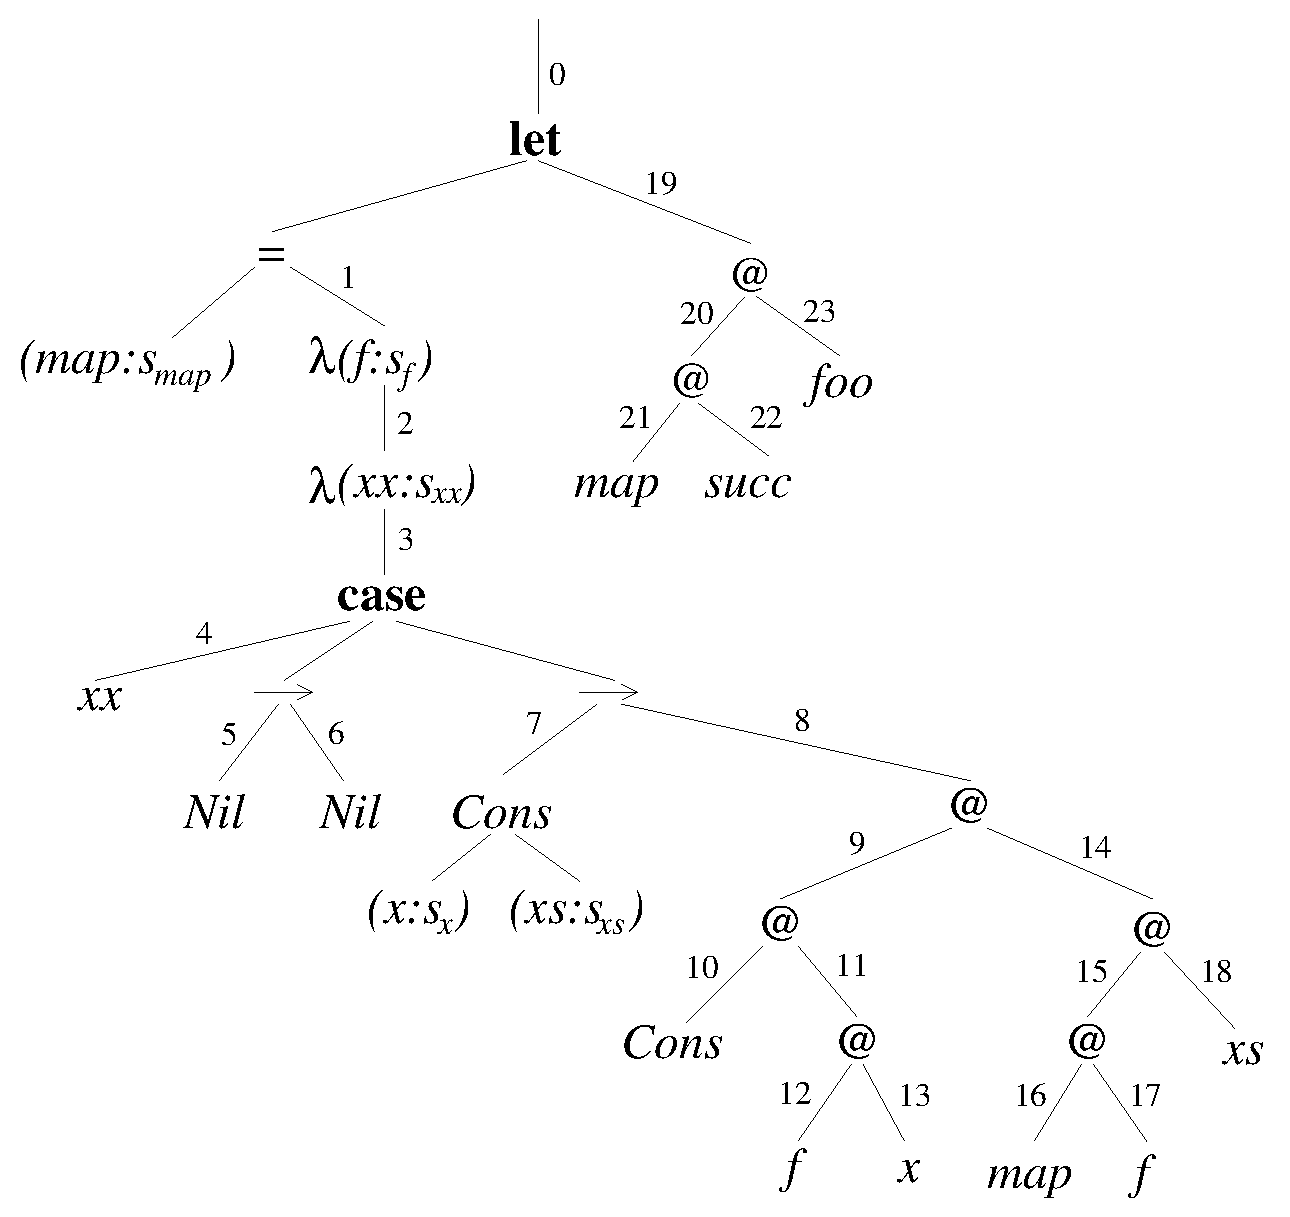
\includegraphics[scale=0.5]{3-Inference/fig/constraints/example-map}
\end{center}

\vspace{8em}
\code{
	$\klet$	& \mc{2}{$(\imap : s_{\imap}) = \lambda (f : s_f). \ \lambda (\ixx : s_{\ixx}).$} \\
		& \ \ $\kcase \ xx \ \kof$							\\
		& \ \ \ \ $\iNil$		& $\to \iNil$					\\
		& \ \ \ \ $\iCons \ (x : s_x) \ (\ixs : s_{\ixs})$
						& $\to \iCons \ (f \ x) \ (\imap \ f \ \ixs)$	\\
	$\kin$	& $\imap \ \isucc \ \ifoo$
}

\clearpage{}
\subsection{Slurping and constraint trees}
\label{Inference:Language:slurping}
In DDC we call the process of extracting type constraints from the annotated syntax tree \emph{slurping} the tree. The function $\rbSLURP$ takes this syntax tree and produces the corresponding constraint tree:

$$
\rbSLURP : \iSyntaxTree \to \iConstraintTree
$$

If the syntax tree has already been annotated with type variables and edge numbers, then the constraints for each node can be produced independently. However, in our implementation we prefer to annotate the tree and generate constraints in a single, bottom-up pass. 

The type constraints extracted from the program's syntax tree are represented by another tree that mirrors its overall shape. We use $\phi$ to represent a branch in this tree, and the branches have the following structure:

\vspace{-1ex}
\begin{tabbing}
MM	\= MM 	\= MM \= MMMMMMMMMMMMMMM \= MMMMMMM \kill
	\> $\phi$ 	\> $\to$ 	\> $\trm{INST} \ x$			
		\> (instantiate this var)		
		\\
\>	\> \ $\mid$	\> $\trm{LAMBDA} \ \ \ov{x} \ \	\ov{\phi}$	
		\> (lambda or case bound var) 		
		\\
\>	\> \ $\mid$	\> $\trm{LET} \ x \ \ 		\ov{\phi}$	
		\> (let bound var) 			
		\\
\>	\> \ $\mid$	\> $\trm{GROUP} \ \ov{x} \ \ 	\ov{\phi}$	
		\> (group of let bindings) 		
		\\
\>	\> \ $\mid$	\> $a = \varphi$
		\> (type equality)			
		\\
\>	\> \ $\mid$	\> $a \tme \varphi$
		\> (effect or closure inequality)
\end{tabbing}

$\rINST \ x$ corresponds to an occurrence of a bound variable in the program source. When extracting constraints we generate an $\rINST \ x$ for every occurrence, irrespective of whether the variable was bound by a let binding, lambda abstraction or pattern match. $\trm{LAMBDA} \ \ov{x} \ \ov{\phi}$ contains constraints arising from a lambda abstraction or pattern match. $\ov{x}$ is the list of bound variables and $\ov{\phi}$ is a list of constraint branches from the body of the abstraction. $\trm{LET} \ x \ \ov{\phi}$ contains constraints arising from a let binding. $\trm{GROUP} \ \ov{x} \ \ov{\phi}$ contains all the constraint branches from a particular mutually recursive let expression. $a = \varphi$ and $a \tme \varphi$ are individual constraints on type variables.

\clearpage{}
% -----------------------------------------------------------------------------
\subsection{Types of programs and declarations}
\label{inference:language:declarations}

\ruleBox{
	\begin{center}
	\fbox{$\Gamma \judge \ipgm :: \varphi$}
	\end{center}
	\begin{gather}
	\ruleI	{Pgm}
		{ \ov{\Gamma \judge \idecl :: \Gamma_d} \quad
		  \Gamma \judge t :: \varphi \quad
		  \Gamma = \Gamma_o, \ov{\Gamma_d}
		}
		{ \Gamma_o \judge \ov{\idecl} \ ; \ t :: \varphi }
	\end{gather}
}
\bigskip
\bigskip

\ruleBox{
	\begin{center}
	\fbox{$\Gamma \judge \idecl :: \Gamma'$}
	\end{center}
	\begin{gather}
	\ruleI	{DeclData}
		{ \ov{\trm{ValidCtor}(T, \ \% \to \ov{\kappa} \to *, \ \varphi)}}
		{ \Gamma \judge 
			\kdata \ T : \% \to \ov{\kappa} \to *  \ 
			\kwhere \ \ov{K : \varphi} \ 
				:: \ (T : \% \to \ov{\kappa} \to *, \ \ov{K : \varphi}) }
	\end{gather}
}

\bigskip
\code{
	\mc{2}{$\trm{ValidCtor}( T, \ \% \to \ov{\kappa} \to *, \ \varphi)$} \\
	 \qq \trm{where}
		& $\varphi = \forall (r : \%) \ \ov{a : \kappa}. \ T \ r \ \ov{a}$
	\\[2ex]
	\mc{2}{$\trm{ValidCtor}( T, \ \% \to \ov{\kappa} \to *, \ \varphi)$} \\
	 \qq \trm{where}
		& $\varphi = \forall (r : \%) \ \ov{a : \kappa}. \ \tau \to T \ r \ \ov{a}$ \\
		& $\ifv(\tau) \setminus \{ r, \  \ov{a} \} \subseteq \emptyset$
	\\[2ex]
	\mc{2}{$\trm{ValidCtor}( T, \ \% \to \ov{\kappa} \to *, \ \varphi)$} \\
	 \qq \trm{where}
		& $\varphi = \forall (r : \%) \ \ov{a : \kappa} \ (c : \$). 
			\ \tau_1 \to \tau_2 \lfuna{c}T \ r \ \ov{a} \ \rhd c \tme x_1 : \tau_1$ \\
		& $(\ifv(\tau_1) \cup \ifv(\tau_2)) \setminus \{ r, \  \ov{a} \} \subseteq \emptyset$
}

\bigskip
In (Pgm), we set the overall type of the program to be the type of its final expression. As data type declarations can be mutually recursive, we add the types and kinds generated by each one to the type environment used when checking them.

In (DeclData) the predicate ValidCtor checks that each constructor has a type appropriate to the data type being declared. We have given the first few cases of ValidCtor, and leave the inductive generalisation to the reader. In our implementation we \emph{generate} the types of data constructors from Haskell style algebraic type definitions, instead of requiring the programmer to give them explicitly, but the checking rules are easier to present.
 
The definition of ValidCtor has several points of note: the type of a constructor cannot have free variables; the type of the return value must have a primary region variable; the types of parameters cannot contain variables that are not present in the return type, and constructors do not have side effects. Also note that the function arrows of constructor types must have appropriate closure annotations, the last case of ValidCtor is an example. This is needed to support the partial application of data constructors.

% -----------------------------------------------------------------------------
\subsection{Kinds of types and constraints}

\ruleBox{
	\begin{center}
	\fbox{ $\varphi :: \kappa$ }
	\end{center}
	\vspace{-1em}
	\begin{gather}
	\ruleA	{KiVar}
		{ a_\kappa :: \kappa }
	\ruleSkip
	\ruleI	{KiConstr}
		{ \varphi :: \kappa \quad
		  \ov{\chi :: \kappa'} \quad
		  \chi \in \Omega
		}
		{ \varphi \rhd \Omega :: \kappa }
	\ruleSkip
	\ruleI	{KiAll}
		{ \varphi :: \kappa' }
		{ \forall(a_{\kappa} : \kappa). \ \varphi :: \kappa' }
	\ruleSkip
	\ruleI	{KiJoin}
		{ \varphi_1 :: \kappa \quad
		  \varphi_2 :: \kappa \quad
		  \kappa \in \{ \ !, \ \$ \ \} 
		}
		{ \varphi_1 \lor \varphi_2 :: \kappa }
	\ruleSkip
	\ruleI	{KiBot}
		{ \kappa \in \{ \ !, \ \$ \ \} }
		{ \bot_{\kappa} :: \kappa }
	\ruleSkip
	\ruleA	{KiTop}
		{ \top_{!} :: \ ! }
	\ruleSkip
	\ruleI	{KiFun}
		{ \tau_1    :: * \quad
		  \tau_2    :: * \quad
		  \sigma    :: \ ! \quad
		  \varsigma :: \$ 
		}
		{ \tau_1 \lfuna{\sigma \ \varsigma} \tau_2 :: * }
	\ruleSkip
	\ruleI	{KiData}
		{ r :: \% \quad
		  \ov{\varphi :: \kappa}
		}
		{ T_{\% \to \ov{\kappa} \to *} \ \ r \ \ \ov{\varphi} :: *}
	\ruleSkip
	\ruleI	{KiRead}
		{ r :: \% }
		{ \iRead \ r :: \ ! }
	\ruleSkip
	\ruleI	{KiReadH}
		{ \varphi :: * }
		{ \iReadH \ \varphi :: \ ! }
	\ruleSkip
	\ruleI	{KiWrite}
		{ r :: \% }
		{ \iWrite \ r :: \ ! }
	\ruleSkip
	\ruleI	{ KiClo }
		{ \varphi :: \kappa \quad
		  \kappa \in \{ \ *, \ \$ \ \} }
		{ (x : \varphi) :: \$ }
	\end{gather}
}

\bigskip
\ruleBox{
	\begin{center}
	\fbox{ $\chi :: \kappa$ }
	\end{center}
	\vspace{-1em}
	\begin{gather}
	\ruleI	{KiCEq}
		{ \tau_1 :: \kappa \quad \tau_2 :: \kappa}
		{ (\tau_1 = \tau_2) :: \kappa }
	\ruleSkip
		\ruleI	{KiCGeq}
		{ \varphi_1 :: \kappa 
		  \quad
		  \varphi_2 :: \kappa 
		  \quad
		  \kappa \in \{ \ !, \ \$ \ \} }
		{ (\varphi_1 \tme \varphi_2) :: \kappa }
	\end{gather}
}

\clearpage{}
Our kinding rules are mostly standard. In (KiConstr) we use the term $\ov{\chi :: \kappa'}$ to require each of the constraints to have a valid kind. The $\chi :: \kappa$ \ judgement ensures that the types on both sides of a constraint have the same kind.


% -----------------------------------------------------------------------------
\subsection{Types of terms}
\begin{center}
	\fbox{$\Gamma \judge t :: \varphi \rhd \Omega \ ; \ \sigma$}
\end{center}


The judgement form $\Gamma \vdash t :: \varphi \ \rhd \ \Omega \ ; \sigma$ reads: ``with environment $\Gamma$ the term $t$ has type $\varphi$, constraints $\Omega$ and effect $\sigma$.'' We will assume that $\varphi$ contains no further constraint sets, and that the typing rules maintain this property. This is a slight abuse of $\rhd$, but we find it more convenient than introducing another operator. Our handling of constraints is based on Leroy's closure typing system \cite{leroy:polymorphic-type-inference}, so the constraint set $\Omega$ is global. When building a type scheme we will include only the constraints reachable from the body of the type. Leroy's approach can be contrasted with Jones's system of qualified types \cite{jones:qualified-types} which encodes constraints as bounds on quantifiers, and uses separate rules to move them between local types and the global set. Our core language uses this second system instead, and we convert between the two representations when translating the source program to core.

In our typing rules we make no attempt to keep the constraint set consistent or satisfiable. Inconsistencies such as $\iInt \ r \ \rhd \iMutable \ r, \ \iConst \ r$ or $\bot \tme \iConsole$ will be discovered when the program is converted to core. The core typing rules ensure that witnesses to the mutability and constancy of a particular region cannot exist in the same program, and effect constraints are checked during type application. Attempting to translate a program that includes inconsistent type constraints to the core language will result in a core type error. However, if these problems are instead detected during type inference, then the compiler would be in a better position to emit a helpful error message. Error handling is discussed in \S\ref{inference:errors}.

The typing rules are presented in three parts, with the static rule in the center, the associated node of the abstract syntax tree on the left, and the generated type constraints on the right. The combination of node and type constraints inductively defines the $\rbSLURP$ function mentioned in \S\ref{Inference:Language:slurping}.

\clearpage{}
% -----
\textbf{Var / Ctor}
$$
\begin{aligned}
	\frac	{x : \forall \ov{a : \kappa}. \ \varphi \rhd \Omega \in \Gamma}
		{\Gamma \judge x :: \varphi[\ov{\varphi'/a}] 
					\rhd \Omega[\ov{\varphi'/a}] \cup \Omega' \ ; \ \bot}
\end{aligned}
$$

\begin{tabbing}
MMMMMMMMMMMMMMMMMMMMM \= MMMMMMMMMMMMM \kill
	\hspace{10em}\includegraphics[scale=0.6]{3-Inference/fig/constraints/var}	
	\> 
	\begin{tabular}{ll}
		$s_1$ 	& $= \rINST \ s_x$ \\
		\\
       	\end{tabular}
\end{tabbing}

We assume that the source program's syntax has already been checked, so $x$ is bound somewhere above its use. The rule for data constructors is identical to the one above, with $x$ replaced by $K$.

The type for $x$ is required to be in the environment, and this type may include quantifiers $\forall \ov{a : \kappa}$ and more constraints $\Omega$. We instantiate this type scheme by substituting new types $\ov{b}$ for the quantified variables in the body of the type as well as its constraints. The extra constraint term $\Omega'$ is needed to match the constraints introduced by other parts of the program, and allows the instantiated type to be weakened and treated as having a larger effect or closure term than it does in the environment. This is required when typing the higher order examples discussed in \S\ref{System:Effects:constraint-strengthening}.

When generating constraints we defer the question of whether the variable was introduced by a let binding, lambda binding, pattern match, or whether it is part of a (mutually) recursive group. If a variable turns out to have been bound by a lambda or pattern match there will be no corresponding generalisation of its type, but we will use $\rINST$ to instantiate it anyway. This makes the resulting constraints easier to read, and simplifies discussion of how to work out the binding dependency graph in \S\ref{inference:ordering}. During type inference we can think of $\rINST$ as a function that blocks on the variable $s_x$, waiting for the type scheme of $x$ to be become available.

\bigskip
% -----
\textbf{Abs}
$$
\begin{aligned}
	& \frac
		{\Gamma, \ x : \tau_1 \rhd \Omega_1 \judge t_2 :: \tau_2 \rhd \Omega_2 \ ; \ \sigma_2}
		{\Gamma \judge \lambda x. \ t_2 \ 
				:: \  \tau_1 \lfuna{e_2 \ c_1} \tau_2 \rhd \Omega_1 \cup \Omega_2 ; \ \bot}
	\\[1ex]
	& \trm{where} \ \ 	\trm{for all} \ y \in \ifv(\lambda x. \ t_2) 
					\ \trm{we have} \ (c_1 \tme y : \Gamma(y)) \in \Omega_2 \\
	& \hspace{7.5ex}	\trm{and} \ e_2 \tme \sigma_2 \in \Omega_2 
\end{aligned}
$$

\begin{tabbing}
MMMMMMMMMMMMMMMMMMM \= MMMMMMMMMMMMM \kill
	\hspace{8em}\includegraphics[scale=0.5]{3-Inference/fig/constraints/lam}
	\> 
	\begin{tabular}{llll}
		\mc{4}{LAMBDA \ $\{ x \}$} \\
			& $s_1$ 	& $= s_x \lfuna{e_2 \ c_1} s_2$ \\
			& $c_1$		& $\tme y_0 : s_{\iyZero} \ \lor \ y_1 : s_{\iyOne} \ \lor \dots$ \\
			&		& $\ \ \ \ \trm{where} \ y_n \gets \ifv(\lambda x. \ t_2)$ 
			\\[1ex]
			& \mc{2}{$\rbSLURP (t_2)$}
		\\ \\ \\ \\
	\end{tabular}
\end{tabbing}

\vspace{-4em}
An abstraction takes a term of type $\tau_1$ and produces a term of type $\tau_2$. When the abstraction is applied it will have the effect $\sigma_2$ of its body. In the typing rule we give this effect the name $e_2$ and bind it to $\sigma_2$ in $\Omega_2$. When generating constraints we can simply annotate the function constructor with $e_2$, and the required effect constraints will be generated when slurping the body. As evaluating the abstraction itself causes no effect, we have $\bot$ in the conclusion of the rule.

The closure of an abstraction contains the types of its free variables. In the typing rule we can read these types directly from the environment using $\Gamma(y)$. When we're generating constraints we won't know what these types are yet, so we use the the place holder variables $s_{\iyZero}, s_{\iyOne} ...$ instead. These variables will be bound to their real types during inference.

\bigskip
% -- App -------------
\textbf{App}

$$
\begin{aligned}
	\frac	{\begin{aligned}
			\Gamma & \judge t_2 :: \tau_3 \lfuna{\sigma_4 \ \varsigma_4} \tau_1 \rhd \Omega
					; \ \sigma_2  \\
			\Gamma & \judge t_3 :: \tau_3 \rhd \Omega \ ; \ \sigma_3 
		 \end{aligned}
		}
		{ \begin{aligned}
		  	\Gamma & \judge t_2 \ t_3 :: \tau_1 \rhd \Omega \ ; \ \sigma_2 \lor \sigma_3 \lor \sigma_4
		  \end{aligned}
		}
\end{aligned}
$$

\begin{tabbing}
MMMMMMMMMMMMMMMMMMMMM \= MMMMMMMMMMMMM \kill
	\hspace{8em}\includegraphics[scale=0.5]{3-Inference/fig/constraints/app}
	\>
	\begin{tabular}{llll}
		$s_2$	& $=	s_3 \lfuna{e_4 \ c_4} s_1$	\\
		$e_1$	& $\tme	e_2 \lor e_3 \lor e_4$ \\[1ex]
		\mc{2}{$e_4, \ c_4$ \trm{fresh}} \\
		\mc{2}{$\rbSLURP(t_2)$} \\
		\mc{2}{$\rbSLURP(t_3)$} \\
		\\ \\ \\ \\
	\end{tabular}
\end{tabbing}

\vspace{-5em}
An application node applies a function of type $\tau_3 \lfuna{\sigma_4 \ \varsigma_4} \tau_1$ to its argument of type $\tau_3$, yielding a result of type $\tau_1$. The act of applying the function has an effect $\sigma_4$. The effect of evaluating the entire expression consists of the effect of evaluating the function value, of evaluating the argument, and of applying the function. In the terminology of \cite{lucassen:polymorphic-effect-systems}, $\sigma_4$ is the \emph{intrinsic} effect of the application and $\sigma_2 \lor \sigma_3$ is the \emph{inherited} effect. The closure of the function is of no consequence when typing an application, so $\varsigma_4$ is only mentioned once in the rule.

When generating type constraints we will not yet know what the effect of the function will be. In our constraints we use $e_4$ and $c_4$ as local names for the function's effect and closure. These will be bound to the actual effect and closure of the function during type inference.

\clearpage{}
% -----
\textbf{Let-Poly}

$$
\begin{aligned}
	\frac	{\begin{aligned}
			\Gamma, \ \ov{x_n : \varphi_n} &  \judge t :: \tau \rhd \Omega \ ; \ \sigma 
			\\
			\Gamma, \ \ov{x_n : \tau_n \rhd \Omega}  
					&  \judge t_0' :: \tau_0' \rhd \Omega \ ; \ \sigma_0'
			\qq \varphi_0 = \rGen(\Gamma, \ \tau_0' \rhd \Omega)
			\\
			\Gamma, \ \ov{x_n : \tau_n \rhd \Omega}  
					&  \judge t_1' :: \tau_1' \rhd \Omega \ ; \ \sigma_1'
			\qq \varphi_1 = \rGen(\Gamma, \ \tau_1' \rhd \Omega) 
			\\
			& \ \vdots \hspace{10em}\ \hspace{4em} \vdots
		 \end{aligned}}
		{\begin{aligned}
			\Gamma & \judge \klet \ \ov{x_n = t_{n}'} \ 	
				\kin \ t :: \tau \rhd \Omega \ ; \ \sigma \lor \sigma_0' \lor \sigma_1' \lor \dots
		 \end{aligned}}
 \end{aligned}
$$

\bigskip
\begin{tabbing}
MMMMMMMMMMMMMMMMMMMMMMM \= MMMMMMMMMMMMM \kill
	\ \ \ \ 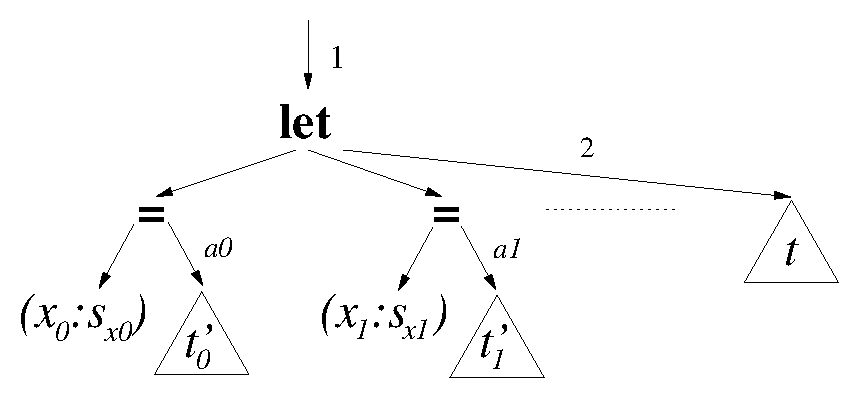
\includegraphics[scale=0.5]{3-Inference/fig/constraints/let}
	\> 
	\begin{tabular}{llll}
		\mc{4}{GROUP $\{ x_0, \ x_1,  \ \dots \}$} \\
			& \mc{3}{$s_1 = s_2$} \\
			& \mc{3}{$e_1 \tme e_{a0} \lor e_{a1} \lor \dots \lor e_2$} 
			\\[1ex]
			& \mc{3}{LET $x_0$} \\	
			&	& $s_{x0} = s_{a0} $ \\
			&	& \textbf{SLURP}($t_0'$) 	\\
			& \mc{3}{LET $x_1$} \\	
			&	& $s_{x1} = s_{a1} $ \\
			&	& \textbf{SLURP}($t_1'$) 	\\
			& \ \ \vdots \\
			& \mc{2}{\textbf{SLURP}($t$)}
 	\end{tabular}
\end{tabbing}

The function Gen generalises the types of each binding. This process is discussed in \S\ref{inference:generalisation}. Note that in the expression:

\code{
	$\varphi = \rGen(\Gamma, \ \tau \ \rhd \Omega)$
}

The resulting type $\varphi$ contains only the constraints from $\Omega$ that are reachable from $\tau$. The conclusion of (Let-Poly) includes the constraint set $\Omega$, and the same set is used in each of the premises. This means that constraints that are conceptually local to a particular binding will ``leak'' into the global set. For example:

$$
	\frac	
	{\begin{aligned}
	 & \Gamma, \ \isuccL : \forall r_1 \ r_2. \ \iInt \ r_1 \to \iInt \ r_2 \rhd \iConst \ r_1 \\
	 & \qq \judge \isuccL \ 3 \\
	 & \qq \ :: \ \iInt \ r_3 \ \rhd \  \iConst \ r_3, \ \iConst \ r_4 \ ; \ \bot
	 \\[1ex]
         & \Gamma, \ \isuccL : \iInt \ r_4 \to \iInt \ r_5 \rhd \iConst \ r_3, \ \iConst \ r_4 \\
	 & \qq \judge \lambda x. \ \isuspendOne \ \isucc \ x  \\
	 & \qq \ :: \ \iInt \ r_4 \to \iInt \ r_5 \rhd \iConst \ r_3, \ \iConst \ r_4 \ ; \ \bot \\[1ex]
	 \end{aligned}
	}
	{\begin{aligned}
	 \Gamma & \judge \klet \ \isuccL = \lambda x. \ \isuspendOne \ \isucc \ 
x \ \kin \ \isuccL \ 3 \\
	 & \ :: \ \iInt \ r_3 \rhd \iConst \ r_3, \iConst \ r_4 \ ; \ \bot
	 \end{aligned}
	}
$$

The function $\isuccL$ is a lazy version of $\isucc$ that reads its argument only when the result is demanded. The general type of $\isuccL$ is:

\code{
	$\isuccL :: \forall r_1 \ r_2. \ \iInt \ r_1 \to \iInt \ r_2 \rhd \iConst \ r_1$
} 

The constraint $\iConst \ r_1$ arises from the use of $\isuspendOne$ in the definition of $\isuccL$. When checking this definition we give $\isuccL$ the monotype:

\code{
	$\iInt \ r_4 \to \iInt \ r_5 \rhd \iConst \ r_4$
}

Due to the formulation of the (Let-Poly) rule, the constraint $\iConst \ r_4$ is actually present in \emph{both} premises, as well as the conclusion. Also, in the body of the let-expression, the application of $\isuccL$ to the constant $3$ requires that constant to be (really) constant, hence the constraint $\iConst \ r_3$. Although this constraint only concerns the body of the let-expression, it is also present in the set used when typing the bindings.

This behavior is unlike that of the (Let) rule presented by Leroy in \cite{leroy:polymorphic-type-inference}. Leroy's rule uses $\rGen$ to split the constraint set arising from a let-binding into two subsets: those that are reachable from the body of the type being generalised, and those that aren't. If we were to use Leroy's approach, the first premise and conclusion of our example would not contain $\iConst \ r_4$, and the second premise would not contain $\iConst \ r_3$. Leroy's rule is ``nicer'' when drawing proof trees, but we stick to the leaky version because it mirrors what happens during type inference. Our inference algorithm adds all the type constraints extracted from the program into a global graph, solves them, then returns the whole graph. It does not section the graph into portions relating to individual bindings, and it only removes constraints from the graph when dealing with the type classes discussed in \S\ref{inference:type-classes}. Retaining information from all bindings also makes it easy for the implementation to add type annotations to the desugared program when converting it to core.

As we have not implemented polymorphic recursion \cite{mycroft:polymorphic-recursion}, we check the right of each binding using the ungeneralised types for each let-bound variable. Due to this, many useful programs are not directly typeable with this (Let-Poly) rule. Consider this example from \cite{mycroft:polymorphic-recursion}:

\bigskip
\qq\qq
\begin{tabular}{lll}
	$\klet$	& \mc{2}{$\imap = \lambda f. \ \lambda \ixx.$}					\\
		& \ \ $\kcase \ xx \ \kof$							\\
		& \ \ \ \ $\iNil$		& $\to \iNil$					\\
		& \ \ \ \ $\iCons \ x \ \ixs$	& $\to \iCons \ (f \ x) \ (\imap \ f \ \ixs)$	
		\\[1ex]
		& $\isquarelist$ & \hspace{-2em} $= \lambda l. \imap \ (\lambda x. \ x * x) \ l$
		\\[1ex]
		& $\icomplement$ & \hspace{-2em} $= \lambda l. \imap \ (\lambda x. \inot x) \ l$
		\\[1ex]
	$\kin$	& \dots
\end{tabular}
\bigskip

This program will not be accepted as it stands. We need to use the generalised, polymorphic type of map when applying it to $(\lambda x. \ x * x)$ and $(\lambda x. \inot x)$ because these expressions have different types. If we use the ungeneralised, monomorphic type then we will get an error.

This highlights the fact that our source typing rules are only a guide for generating type constraints, and that we cannot use them to check the source program directly. We must first perform type inference by extracting type constraints and then solving them. As discussed in \S\ref{inference:ordering}, our algorithm for solving type constraints also builds a graph that records what bindings are mutually recursive. Once we have this graph we can use it to split out the definition of $\imap$ from the above example, and convert the program to:

\bigskip
\qq\qq
\begin{tabular}{lll}
	$\klet$	& \mc{2}{$\imap = \lambda f. \ \lambda \ixx.$}					\\
		& \ \ $\kcase \ xx \ \kof$							\\
		& \ \ \ \ $\iNil$		& $\to \iNil$					\\
		& \ \ \ \ $\iCons \ x \ \ixs$	& $\to \iCons \ (f \ x) \ (\imap \ f \ \ixs)$	
		\\[1ex]
	$\kin$ \\
	$\klet$	& $\isquarelist$ & \hspace{-2em} $= \lambda l. \imap \ (\lambda x. \ x * x) \ l$
		\\[1ex]
		& $\icomplement$ & \hspace{-2em} $= \lambda l. \imap \ (\lambda x. \inot x) \ l$
		\\[1ex]
	$\kin$	& \dots
\end{tabular}

\bigskip
For this version, (Let-Poly) allows us to use the generalised type of $\imap$ when checking the body of the second let-expression. This new program will be accepted without error.

% The effect of the whole expression includes the effects $\sigma_0, \sigma_1, \dots$ of its bindings along with the effect $\sigma$ of the body. The structure of the constraints mirrors that of the original expression. \trm{GROUP} signals that the enclosed constraints contain a refer to a set of (mutually) recursive $\klet$ bindings, and \trm{LET} denotes the scope of each one. 

\bigskip
% ----------
\textbf{Case}
$$
\begin{aligned}
	\frac	
	{\begin{aligned}
		\begin{aligned}
		  \\ \\ \\
		  \Gamma & \judge t :: T \ r \ \ov{\varphi} \rhd \Omega \ ; \ \sigma 
		\end{aligned}
		&
		\begin{aligned}
		  \Gamma & \judgea{p} p_0 \to t_0' :: T \ r \ \ov{\varphi} \to \tau \rhd \Omega \ ; \ \sigma_0' \\
		  \Gamma & \judgea{p} p_1 \to t_1' :: T \ r \ \ov{\varphi} \to \tau \rhd \Omega \ ; \ \sigma_1' \\
		 	 & \hspace{6em} \vdots
	 	\end{aligned}
	 \end{aligned} 
	}
	{\begin{aligned}
	  \Gamma  & \judge \kcase \ t \ \kof \ \ov{p \to t'} :: \tau' \rhd \Omega
				\ ; \ \iRead \ r \lor \sigma \ \lor \sigma_0' \lor \sigma_1' \lor \dots
	 \end{aligned}
	}
 \end{aligned}
$$

\begin{tabbing}
	MMMMMMMMMMMMMMMMMMM \= MMMMMMMMMMMMM \kill
	\hspace{1em}\includegraphics[scale=0.5]{3-Inference/fig/constraints/case} 
	\> \begin{tabular}{lll}
		$s_2$ 	& $= s_{p0}$ \\
		$s_2$	& $= s_{p1}$ \\
			& \ \ \vdots \\
		$s_1$	& $= s_{a0}$ \\
		$s_1$	& $= s_{a1}$ \\
			& \ \ \vdots \\
		$e_1$	& $= \iReadH s_2 \lor e_2 \lor e_{a0} \lor e_{a1} \lor \dots$ \\
		\mc{2}{$\rbSLURP(t)$} \\
		\mc{2}{$\rbSLURP(p_0)$} \\
		\mc{2}{$\rbSLURP(p_1)$} \\
			& \ \ \vdots \\
		\mc{2}{$\rbSLURP(t_0)$} \\
		\mc{2}{$\rbSLURP(t_1)$} \\
			& \ \ \vdots \\
		\\ \\ \\ \\ \\ \\ 
	    \end{tabular}
\end{tabbing}

\vspace{-8em}

A case expression requires the discriminant $t$ to have the same type as the patterns being matched against. For all alternatives, the types of the patterns must be identical, and so must the types of the expressions. The type of the entire case expression is the type of the right of the alternatives. 

The effect of a case expression includes the effect of evaluating the discriminant and examining it, as well as evaluating the alternatives. When type checking a program in a bottom-up manner, when it's time to apply the (Case) rule we will already know the type of the discriminant. In this situation we can use $\iRead \ r$ as the effect of examining it. On the other hand, when generating constraints we will not yet know the type of the discriminant. We instead use $\iReadH s_2$, which represents a read effect on the primary region of the (currently unknown) type $s_2$. During inference, the type of $s_2$ will resolve to the real type of the discriminant. After this is done, $\iReadH s_2$ can be reduced to a $\iRead$ effect on the primary region of this new type.

\clearpage{}
\ruleBox{
	\begin{center}
	\fbox{ $\Gamma \judgea{p} p \to t :: \tau_1 \to \tau_2 \rhd \Omega$ }
	\end{center}
	\vspace{-1em}
	\begin{gather}
	\ruleI	{Pat-Wildcard}
		{ \Gamma \judge t :: \tau_2 \rhd \Omega \ ; \ \sigma }
		{ \Gamma \judgea{p} \_ \to t :: \tau_1 \to \tau_2 \rhd \Omega \ ; \ \sigma }
	\ruleSkip
	\ruleI	{Pat-Constructor}
		{ 	T & : \% \to \ov{\kappa} \to * \in \Gamma
			\\
			K & : \forall (r : \%) \ \ov{a : \kappa} \ \ov{c : \$}
				. \ \ov{\tau} \lfuna{c'} T \ r \ \ov{a} \ \rhd \Omega \in \Gamma 
			\qq \theta = [\ r' / r \ \ \ov{\varphi/a} \ ]
			\\
	  		& \Gamma, \ \ov{x_n : \theta(\tau_n) \ \rhd \ \theta(\Omega)}^{\: n}
				\judge t :: \tau' \rhd \Omega' \ ; \ \sigma
		}
		{ \Gamma \judgea{p} K \ \ov{x} \to t 
			:: T \ r' \ \ov{\varphi} \to \tau' \rhd \Omega' \ ; \sigma }
	\end{gather}
}
\bigskip
\begin{tabbing}
	MMMMMMMMMMMMMMMMM \= MMMMMMMMMMMMM \kill
	\hspace{6em}\includegraphics[scale=0.5]{3-Inference/fig/constraints/pat} 
	\> $\begin{aligned}
		s_1 & = T \ r' \ \ov{a'} \\
		s_x & = \tau' \\
		\vdots \\
                & \trm{where} \ \tau' \to \dots \to T \ r' \ \ov{a'}\\
		& \hspace{2em}  = \trm{Inst}(\forall (r : \%) \ \ov{a : \kappa} \ \ov{c : \$}
					. \ \ov{\tau} \lfuna{c'} T \ r \ \ov{a})
		\\ \\ \\
	    \end{aligned}$
\end{tabbing}

\vspace{-2em}
The judgement form $\Gamma \judgea{p} p \to t :: \tau_1 \to \tau_2 \rhd \Omega$ reads: ``with environment $\Gamma$ an alternative matching a pattern $p$ and producing a term $t$ has type $\tau_1$ to $\tau_2$ with constraints $\Omega$.''

Matching against a wildcard produces no constraints.

In (Pat-Constructor) we lookup the type of the constructor $K$ from the environment. The (DeclData) rule from \S\ref{inference:language:declarations} introduces these types into the environment and ensures that they have the particular form shown here.

The variables bound by the pattern are named $\ov{x}$, and the types of these variables must have the same form as the types of the arguments of the constructor. If the constructor produces a type containing variables $\ov{a}$ then all occurrences of $\ov{x}$ must agree on the particular types used for $\ov{a}$. For example with the constructor:

\code{
	$\iCons :: \forall r \ a \ c. \ a \to \iList \ r \ a \lfuna{c} \iList \ r \ a \ \rhd \ c \tme x : a$
}

Consider the alternative in:

\code{
	$\kcase \ \dots \ \kof$ \\
	\ \ $\iCons \ x \ \ixs \to \dots$
}

We cannot, say, use $x$ at type $\iInt \ r_1$, but $\ixs$ at type $\iCons \ r_2 \ (\iBool \ r_1)$ because $\iInt \ r_1 \ \neq \ \iBool \ r_1$. This restriction is achieved by requiring the types of each of the pattern bound variables to be related by the substitution $\theta$.

The constraint generation rules given here only concern the pattern in a particular alternative. The job of matching up the types of all alternatives in a case-expression is handled by the constraints for the (Case) rule on the previous page. 

When generating constraints for a pattern, we first take a fresh instance of the constructor's type scheme. The result type is the type of the overall pattern, and the argument types are assigned to the variables bound by the pattern.



